\chapter{Planificación del proyecto}\label{ch:planificacion}
En esta sección se incluyen los aspectos relativos a la planificación del proyecto.
Incluyendo un test de viabilidad, planificación temporal, diagrama de Gantt y el presupuesto asociado al
trabajo.


\section{Test de viabilidad}\label{sec:test-de-viabilidad}
Se realiza tests de viabilidad para comprobar la factibilidad del proyecto.

Dando lugar al desarrollo de una primera prueba que consistió en la extracción de cortes del plano axial de un pequeño
set de biomarcadores MRI, que se incluyeron como datos de entrenamiento de una red neuronal básica de prueba y del que
se comprobó que era posible obtener una clasificación del grado del Alzheimer presente en una MRI a partir de uno de
los planos cerebrales.

Y una segunda prueba en la que integró un modelo de DL de clasificación de imágenes en una pequeña aplicación web
usando Flask y en la que se comprobó que era posible la integración.

Por lo tanto, los resultados satisfactorios de ambas pruebas concluyeron que la realización de este proyecto era viable.


\section{Planificación temporal}\label{sec:planificacion-temporal}
La planificación de este proyecto se divide en tres fases:
\begin{itemize}
    \item Una primera fase de investigación exhaustiva en la que se realiza un estudio de los conceptos teóricos de la
    EA y de las herramientas de DL y de procesamiento de imágenes de la literatura de este ámbito y en la que se obtiene
    una conclusión al estado del arte.
    \item Una segunda fase en la que se realiza la experimentación correspondiente al desarrollo del sistema de DL y al
    desarrollo de la aplicación web.
    \item Una tercera fase en la que concluyen los resultados finales obtenidos. \\
\end{itemize}

Cabe destacar que la fase de investigación perdura en el tiempo, ya que, durante la primera parte se realiza una
investigación más exhaustiva de la literatura, pero durante el desarrollo de todo el proyecto es necesario consultar
información.

Como se puede ver en el Diagrama de Gantt, sección~\ref{sec:diagrama-de-gantt} la planificación está separada temporalmente por
3 meses en los cuales se produce un parón en la realización del trabajo.
De manera que, la duración aproximada del proyecto es de 5 meses, comenzando del 1 de marzo al 6 de mayo, donde comienza
el parón, y reanudándose el 5 de agosto hasta la fecha límite del 16 de noviembre.

\subsection{Planificación}\label{subsec:planificacion}
Como se ha comentado en el apartado~\ref{subsec:metodologia}, para completar el proyecto se han definido un conjunto
de \textit{milestones} que engloban los objetivos asociados al trabajo.
Esos \textit{milestones} pertenecen a las siguientes etapas de realización:

\subsubsection{Preparación del proyecto}
El \textit{milestone} \textbf{1. Base e introducción} se integra en esta etapa en la que se realiza la investigación de
la literatura necesaria correspondiente al ámbito del problema y además se incluye la preparación del entorno y del
sistema de trabajo.

\subsubsection{Desarrollo}
Los \textit{milestones} \textbf{2. Análisis y Desarrollo experimental} y \textbf{3. Desarrollo de la aplicación web} se
incluyen en la fase de desarrollo.
Por lo tanto, se incluye en esta fase:

\begin{itemize}
    \item El procesamiento de los biomarcadores.
    \item La creación de los dataset de entrenamiento.
    \item El desarrollo del algoritmo de aprendizaje profundo.
    \item La especificación de la aplicación web.
    \item El proceso de diseño de la aplicación web.
    \item El desarrollo de la aplicación web.
    \item El testeo de la aplicación web.
    \item La conclusión al trabajo realizado. \\
\end{itemize}
Es la fase que conlleva más tiempo y en la que cabe destacar que ambas partes de desarrollo, el sistema de DL y la
aplicación web, se realizan en paralelo y que, para su finalización, la aplicación web requiere de la finalización de
la parte del desarrollo de sistema de DL, ya que hace uso de él.

De manera que la aplicación web comienza su desarrollo de manera independiente al principio, esperando a que se complete
el desarrollo experimental del sistema de DL para poder integrarlo.

\subsubsection{Conclusión}
Una vez completada la etapa de desarrollo se puede realizar la comparativa de los resultados del desarrollo experimental
y se puede completar la conclusión final del proyecto.

En esta tabla se muestra el tiempo dedicado a las diferentes tareas anteriormente comentadas:

\begin{table}[H]
    \centering
    \begin{tabular}{|l|l|}
        \hline
        \textbf{Tarea} & \textbf{Tiempo (horas)} \\
        \hline
        Test de viabilidad & 24 \\
        \hline
        Planificación & 80 \\
        \hline
        Investigación de la literatura & 100 \\
        \hline
        Preparación del entorno & 8 \\
        \hline
        Procesamiento de biomarcadores & 20 \\
        \hline
        Creación de los dataset de entrenamiento & 40 \\
        \hline
        Desarrollo del algoritmo de aprendizaje profundo & 160 \\
        \hline
        Especificación de la aplicación web & 8 \\
        \hline
        Diseño de la aplicación web & 8 \\
        \hline
        Desarrollo de la aplicación web & 40 \\
        \hline
        Testeo de la aplicación web & 8 \\
        \hline
        Conclusión del desarrollo & 24 \\
        \hline
        \hline
        Total & 520 \\
        \hline
    \end{tabular}
    \caption{Planificación temporal}
    \label{tab:tabla_planificacion_temporal}
\end{table}

\section{Diagrama de Gantt}\label{sec:diagrama-de-gantt}

\begin{figure}[H]
    \centering
    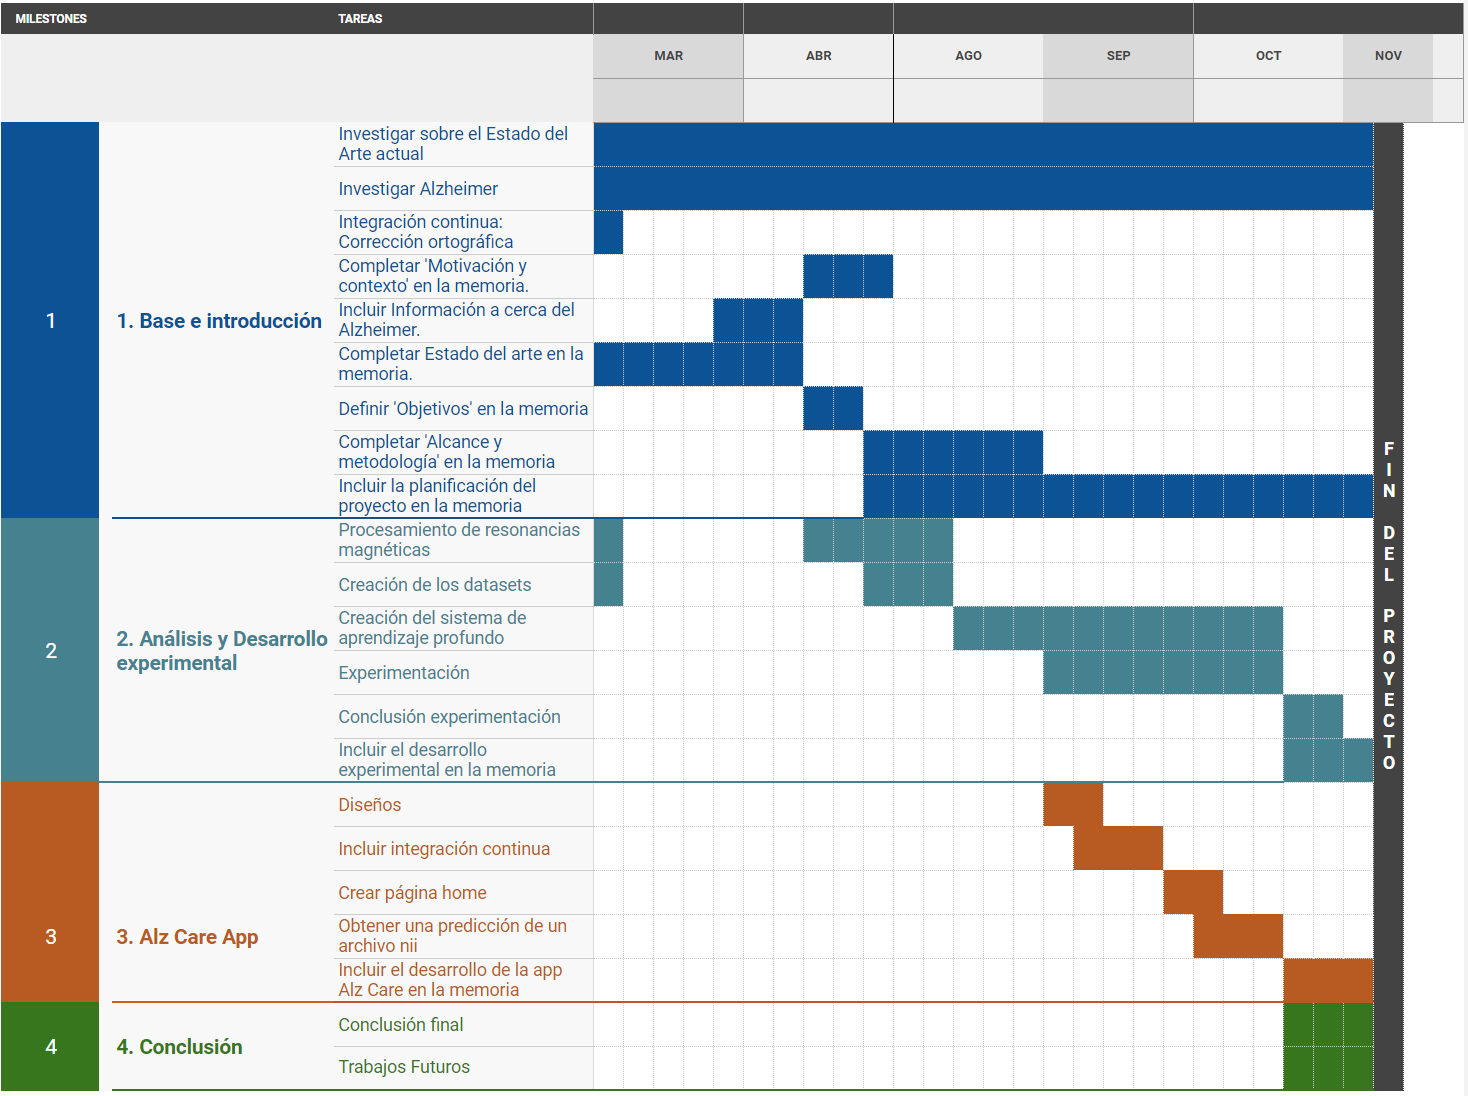
\includegraphics[width=\textwidth]{./imgs/diagrama-gantt}
    \caption{Diagrama de Gantt}
    \label{fig:diagrama-gantt}
\end{figure}

\section{Presupuesto}\label{sec:presupuesto}
Se dividen tres tipos de recursos para llevar a cabo las tareas del proyecto: recursos humanos, de software y de
hardware, de manera que el presupuesto se realiza basándose en estos tres tipos de recursos.

\subsection{Recursos humanos}\label{subsec:recursos-humanos}
Los recursos humanos necesarios para realizar el proyecto se han dividido según el rol que desempeñan en el mismo
y se muestran en la siguiente tabla:

\begin{table}[H]
    \centering
    \begin{tabular}{|l|l|l|l|}
        \hline
        \textbf{Rol} & \textbf{Precio por hora (euros/hora)} & \textbf{Tiempo (horas)} & \textbf{Coste (horas)} \\
        \hline
        Manager & 15.5 & 188 & 2914 \\
        \hline
        Investigador & 10.5 & 100 & 1050 \\
        \hline
        Analista & 9 & 24 & 216 \\
        \hline
        Diseñador & 10.5 & 8 & 84 \\
        \hline
        Programador & 10.5 & 192 & 2016 \\
        \hline
        Tester & 9 & 8 & 72 \\
        \hline
        \hline
        Total & & 520 & 6352 \\
        \hline
    \end{tabular}
    \caption{Recursos humanos}
    \label{tab:tabla_recursos_humanos}
\end{table}

\subsection{Recursos software}\label{subsec:recursos-software}
Los recursos software y su coste se incluyen en la siguiente tabla:

\begin{table}[H]
    \centering
    \begin{tabular}{|l|l|l|}
        \hline
        \textbf{Tipo} & \textbf{Recurso} & \textbf{Coste (euros)} \\
        \hline
        Sistema Operativo & Linux & 0 \\
        \hline
        IDE & Visual Studio Code & 0 \\
        \hline
        IDE & IntelliJ IDEA & 0 \\
        \hline
        \hline
        Total &  & 0 \\
        \hline
    \end{tabular}
    \caption{Recursos software}
    \label{tab:tabla_recursos_software}
\end{table}

\subsection{Recursos hardware}\label{subsec:recursos-hardware}
Los recursos hardware y su coste teniendo en cuenta que se van a amortizar durante 5 meses
se incluyen en la siguiente tabla:

\begin{table}[H]
    \centering
    \begin{tabular}{|l|l|l|l|l|}
        \hline
        \textbf{Recurso} & \textbf{Modelo} &  \textbf{Coste (€)} & \textbf{Vida útil} & \textbf{Amortización (€)} \\
        \hline
        Portátil & HP-Pavilion 15-cs0xxx & 1350 & 5 años & 140.63 \\
        \hline
        Entornos de G.Colab &  & 0 & & 0 \\
        \hline
        \hline
        Total &  & 1350 &  & 140.63 \\
        \hline
    \end{tabular}
    \caption{Recursos hardware}
    \label{tab:tabla_recursos_hardware}
\end{table}


\subsection{Presupuesto final}\label{subsec:presupuesto-final}
A partir del presupuesto de los recursos asociados a la realización del proyecto se muestra el presupuesto total final
en la siguiente tabla:

\begin{table}[H]
    \centering
    \begin{tabular}{|l|l|}
        \hline
        \textbf{Tipo} & \textbf{Coste (euros)} \\
        \hline
        Recursos Humanos & 6352 \\
        \hline
        Recursos Software & 0 \\
        \hline
        Recursos Hardware & 140.63 \\
        \hline
        \hline
        Total & 6492.63 \\
        \hline
    \end{tabular}
    \caption{Presupuesto final}
    \label{tab:tabla_presupuesto_final}
\end{table}